\documentclass[12pt,
border=1pt]{standalone}
\usepackage{pgfplots}
\usepackage{amsmath}
\usepackage{amssymb}

\pgfplotsset{compat=newest,
	width=6cm, height=5cm,
	xtick pos=left, ytick pos=left,
	%            scaled x ticks=real:1e-6,
}
% Kernel 2 FP64
\begin{document}
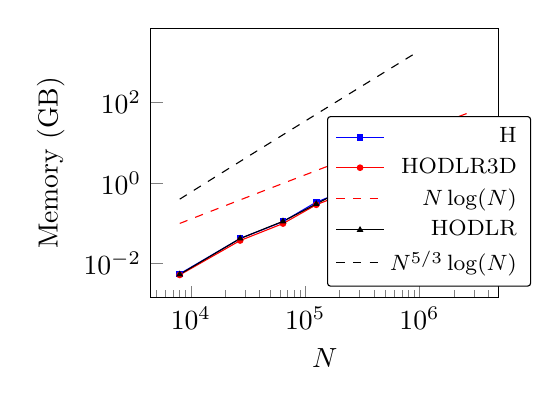
\begin{tikzpicture}[every mark/.append style={mark size=1pt}]
	\begin{axis}[xlabel={$N$},
	ylabel={Memory (GB)},
%		legend pos=south east,
		legend style={
                at={(0.8,0.04)},
               anchor=south,
               legend columns=1,
               cells={anchor=east},
              font=\footnotesize,
               rounded corners=1pt,
               },
		xmode = log,
	    ymode = log,
	   % xmin = 1e3,
	   % xmax = 1e6,
	   % ymin = 1e-10,
	   % ymax = 1e-0,
	   % xtick={1e-10, 1e-8, 1e-6,  1e-4,  1e-2},
	   % ytick={1e-8, 1e-6,  1e-4,  1e-2, 1e-0}
		]
		
		\addplot[
		color=blue,
		mark=square*,
		] coordinates {
(8000,0.005555)
(27000,0.041799)
(64000,0.109662)
(125000,0.332887)
(216000,0.610886)
(343000,1.014650)
(512000,1.553900)
(729000,2.349640)
(1000000,4.129140)
(1331000,5.671150)
(1728000,7.456180)
		};
		\addplot[
		color=red,
		mark=*,
		] coordinates {
(8000,0.005215)
(27000,0.037240)
(64000,0.098029)
(125000,0.286593)
(216000,0.529518)
(343000,0.882407)
(512000,1.354990)
(729000,2.041050)
(1000000,3.516390)
(1331000,4.828830)
(1728000,6.386160)
(2197000,8.301580)
(2744000,10.511400)
		};
		\addplot[mark=none, red, dashed][
		domain = 8000:2744000,
		] {(pow(10,-5.5)*x*log10(x)};
\addplot[
		color=black,
		mark=triangle*,
		] coordinates {
% (8000,0.003738)
% (27000,0.021623)
% (64000,0.070984)
% (125000,0.183103)
% (216000,0.393824)
% (343000,0.783232)
% (512000,1.344510)
% (729000,2.171780)
% (1000000,3.574900)
% (1331000,5.7101)
(8000,5.395010e-03)
(27000,4.179560e-02)
(64000,1.113700e-01)
(125000,2.998880e-01)
(216000,6.762740e-01)
(343000,1.336920e+00)
(512000,2.465660e+00)
(729000,4.231330e+00)
(1000000,6.965400e+00)
		};
\addplot[mark=none, black, dashed][
		domain = 8000:1000000,
		] {(pow(10,-7.5)*pow(x,5/3)*log10(x)};
		\legend{H, HODLR3D, $N\log(N)$, HODLR, $N^{5/3}\log(N)$}	
% \legend{H, HODLR3D, HODLR}
		\end{axis}
\end{tikzpicture}
\end{document}